% This must be in the first 5 lines to tell arXiv to use pdfLaTeX.
\pdfoutput=1

% =========================
% main.tex
% OUTDATED early preprint draft — superseded by the anonymized workshop
% submission. Numbers and claims here predate the expanded runs; do not cite.
% =========================

\documentclass{article}

% Match prior paper formatting package/layout.
\usepackage[preprint]{neurips_2026}

\usepackage[T1]{fontenc}
\usepackage[utf8]{inputenc}
\IfFileExists{microtype.sty}{\usepackage{microtype}}{}
\usepackage{amsmath,amssymb}
\usepackage{booktabs}
\IfFileExists{multirow.sty}{\usepackage{multirow}}{}
\usepackage{graphicx}
\usepackage{xcolor}
\IfFileExists{enumitem.sty}{%
  \usepackage{enumitem}
}{%
  \let\oldenumerate\enumerate
  \let\endoldenumerate\endenumerate
  \renewenvironment{enumerate}[1][]{\oldenumerate}{\endoldenumerate}
}
\IfFileExists{caption.sty}{\usepackage{caption}}{}
\IfFileExists{subcaption.sty}{\usepackage{subcaption}}{}
\usepackage{array}
\usepackage{float}
\usepackage{hyperref}
\usepackage{pgfplots}
\pgfplotsset{compat=1.18}
\usepgfplotslibrary{groupplots}
\usetikzlibrary{arrows.meta,positioning,fit}

\title{Latent-State Auditing for Tool-Using Language Agents}

\author{
Anonymous Authors \\
Anonymized for review
}

\begin{document}

\maketitle

\begin{abstract}
Tool-using language agents are vulnerable to indirect prompt injection because untrusted external content can change which tools an agent chooses and how it uses them. Existing agent-security evaluations primarily observe the outside of this process: prompts, transcripts, tool calls, tool results, and final task outcomes. This paper studies whether those evaluations can be minimally augmented with an internal measurement: activation-derived evidence at the decision points immediately before tool use. We introduce latent-state auditing, a pipeline that captures residual-stream activations at security-critical trajectory points, verbalizes them with Natural Language Autoencoders (NLAs), maps the resulting explanations into a latent-risk taxonomy, and trains cheap monitors that can be compared against transcript and tool-policy baselines. In AgentDojo-grounded replay experiments with Qwen2.5-7B and a released Qwen NLA activation verbalizer, raw keyword labels over NLA text are weak, but trained NLA-text and raw-activation monitors strongly separate attacked from clean records, including held-out suite and attack-template splits. In model-generated next-action trajectories, Qwen produces 22 unsafe tool actions in an AgentDojo important-instructions slice; learned latent monitors flag all 22 before the generated unsafe execution step, with mean lead time near two steps. These results do not show that NLAs are faithful mind readers or production firewalls. They support a narrower claim: activation-grounded auditing adds a useful internal-state measurement axis to agent-security evaluations, and expensive NLA explanations can serve as forensic evidence and weak supervision for cheaper runtime probes.
\end{abstract}

\section{Introduction}

Language agents are increasingly built around tools. They read email, browse webpages, inspect repositories, manage calendars, query databases, write files, and call external APIs. This tool access is what makes agents useful, but it also changes the security problem. A chatbot can produce a harmful answer; a tool-using agent can send an email, delete a file, exfiltrate data, modify a calendar, or execute code. In these settings, the dangerous moment is often not the final response. It is the internal decision immediately before tool selection or tool execution.

Indirect prompt injection exploits exactly this boundary. A user gives a trusted instruction, but the agent then observes attacker-controlled external content: an email body, a webpage, a document, a repository issue, a tool result, or a tool description. The attack succeeds when the agent treats that untrusted content as an instruction and calls a tool for the attacker rather than for the user. Agent-security benchmarks have made this failure concrete. AgentDojo evaluates prompt-injection attacks and defenses in a dynamic tool environment with realistic task suites and security cases \citep{agentdojo2024}. InjecAgent studies indirect prompt injection in tool-integrated agents across more than one thousand cases and distinguishes direct harm from private-data exfiltration \citep{injecagent2024}. ToolHijacker shows that the tool-selection layer itself is attackable: malicious tool documentation can steer retrieval and final tool choice \citep{toolhijacker2025}. ToolEmu and AgentHarm broaden the evaluation landscape to high-stakes tool risk and explicitly harmful multi-step agent behavior \citep{toolemu2024,agentharm2025}.

These evaluations are essential, but they mostly measure what is externally visible. They record the task, attack, transcript, selected tool, tool arguments, and outcome. That is enough to say whether the agent failed. It is not enough to answer a different question: was the failure already detectable inside the model before the unsafe tool action became visible? For agent security, this question matters because some interventions must happen before execution. A monitor that first notices danger after \texttt{send\_email}, \texttt{delete\_file}, or \texttt{run\_shell} is less useful than one that flags the decision state immediately before the call.

This paper studies latent-state auditing as a minimal augmentation to existing agent-security evaluations. The proposal is deliberately narrow. We do not replace AgentDojo, InjecAgent, ToolHijacker, CaMeL-style capability control, or tool-policy checks. Instead, for the same benchmark cases and decision points, we add one internal measurement:
\[
(\text{case}, \text{trajectory}, \text{decision point}) \rightarrow \text{activation} \rightarrow \text{NLA text} \rightarrow \text{latent labels and probe scores}.
\]
The resulting question is empirical: do activation-derived signals predict unsafe future tool use earlier or differently than transcript and tool-policy baselines?

Natural Language Autoencoders (NLAs) make this measurement possible in a form that is directly inspectable. An NLA consists of an activation verbalizer, which maps a residual-stream activation to a natural-language explanation, and an activation reconstructor, which maps the explanation back to an activation \citep{anthropic2026nla}. The method is trained for activation reconstruction rather than supervised explanation labels, and Anthropic reports that NLA explanations can surface safety-relevant latent information such as unverbalized evaluation awareness. At the same time, the NLA paper is explicit about limitations: explanations can confabulate, lack mechanistic grounding, over-infer because the verbalizer is itself a language model, and are expensive to run at scale \citep{anthropic2026nla}. Those limitations determine the design of this work. We use NLA output as noisy audit evidence and weak supervision, not as ground truth and not as a production firewall.

Our empirical story has three stages. First, synthetic development runs established the full pipeline and exposed an important negative result: raw keyword labels over NLA text were noisy, while raw activation probes often contained a stronger separable signal. Second, AgentDojo-grounded replay experiments with Qwen2.5-7B and the released Qwen layer-20 NLA activation verbalizer produced strong trained NLA-text and raw-activation results, including held-out suite and attack-template transfer. Third, and most importantly, model-generated next-action trajectories produced actual unsafe Qwen tool actions under an AgentDojo important-instructions slice. In the larger generated-action run, Qwen generated 22 unsafe tool actions, consisting of 13 \texttt{send\_email} calls and 9 \texttt{delete\_file} calls. Learned latent monitors flagged all 22 before the generated unsafe execution step, with mean lead time of 2.00 steps for the raw activation probe and 1.95 steps for the trained NLA-text monitor.

The correct interpretation is not that latent monitors dominate ordinary tool policy. In the generated-action slice, a tool-policy baseline trivially catches the unsafe action once the generated tool call is visible. The value of latent monitoring is earlier and more diagnostic: it provides evidence at pre-action states, before the execution event. This makes latent-state auditing a complement to least privilege, capability control, sandboxing, provenance tracking, and tool authorization. It is an additional measurement axis for evaluations, not a replacement security architecture.

Our contributions are as follows:
\begin{enumerate}[leftmargin=1.5em]
    \item We introduce latent-state auditing as a thin instrumentation layer for existing agent-security evaluations, capturing activations and NLA explanations at security-critical decision points without changing the benchmark task semantics.
    \item We define a latent-risk taxonomy for tool-using agents, covering external instruction internalization, attacker-goal activation, unauthorized tool intent, tool-selection hijacking, private-data targeting, control-flow contamination, and monitor evasion.
    \item We implement an end-to-end evaluation scaffold over AgentDojo-style records, including export, prompt-provenance tracking, Qwen activation capture, local NLA verbalization, latent labeling, trained NLA-text monitoring, raw activation probing, hybrid scoring, complementarity, calibration, and lead-time summaries.
    \item We report replay and model-generated action evidence. In replay, trained NLA-text and raw activation monitors transfer across held-out suites and attack templates. In generated-action trajectories, learned latent monitors flag all 22 Qwen-generated unsafe actions before execution.
    \item We give a claim-hygiene framework that separates mock tests, normalized replay, exact-prefix replay, proxy lead-time, and model-generated action evidence, and we document negative results where raw NLA keyword labels fail.
\end{enumerate}

\section{Related Work}

\subsection{Agent-security benchmarks}

AgentDojo is the closest benchmark substrate for this work. It frames prompt injection as an agent problem: data returned by external tools can hijack an agent into performing a malicious side task, and defenses must preserve both utility and security \citep{agentdojo2024}. Its dynamic environment, task suites, injection tasks, and utility-under-attack metrics make it a natural place to add latent telemetry. Our use of AgentDojo is intentionally conservative. We do not modify its threat model or claim a new benchmark; we export AgentDojo-grounded cases and add activation/NLA observations at the same decision points where the agent is about to choose or execute a tool.

InjecAgent provides a complementary formulation of indirect prompt injection in tool-integrated agents \citep{injecagent2024}. It contains 1,054 test cases across 17 user tools and 62 attacker tools, and categorizes attacks into direct harm and private-data exfiltration. This taxonomy is important for latent-state auditing because it suggests labels that are more specific than a binary attacked/clean distinction. A latent explanation that indicates private-data targeting, unauthorized transmission, or direct-harm intent is more useful for forensics than a generic anomaly score.

ToolHijacker shifts attention from tool execution to tool selection \citep{toolhijacker2025}. In many agent systems, tool use involves retrieval over tool descriptions followed by final selection. ToolHijacker shows that malicious tool documents can manipulate this process and that several existing defenses are insufficient. This motivates auditing not only the final tool call but also earlier points: before retrieval, after tool documentation is inserted, and before final selection. Our current experiments focus on before-selection and before-execution states, but the pipeline is designed to support those ToolHijacker-style hooks.

ToolEmu studies a different bottleneck: scalable safety testing for agents with high-stakes tools \citep{toolemu2024}. It uses language models to emulate tool execution and evaluate safety/helpfulness, enabling risk assessment over 36 high-stakes toolkits and 144 test cases. ToolEmu's separation between scenario generation, tool emulation, and safety evaluation is methodologically close to our separation between benchmark generation and latent auditing. NLAs are too expensive to run everywhere; a practical workflow can use broad scenario generation or behavioral evaluators to find suspicious subsets, then apply latent audits to those cases.

AgentHarm evaluates explicitly harmful multi-step agent tasks rather than indirect attacks through external data \citep{agentharm2025}. It contains 110 base malicious behaviors, 440 augmented tasks, 11 harm categories, and 104 tools. Its key lesson for this paper is that agent safety is not reducible to single-turn refusal. A harmful agent must maintain enough capability to carry out multi-step tool use. Latent-state auditing is aimed at this same pre-action regime: when a capable model is planning or selecting tools, can a monitor detect risk before the harmful sequence completes?

\subsection{Capability control and secure-by-design agents}

The strongest defenses against prompt injection try to prevent untrusted data from influencing control flow in the first place. CaMeL is the clearest example: it extracts control and data flow from trusted queries, prevents untrusted data from altering program flow, and uses capabilities to restrict unauthorized exfiltration \citep{camel2025}. This paper should be read as complementary to that line of work. Latent-state auditing does not provide the same kind of design-time guarantee. Instead, it can help evaluate and diagnose the residual cases where a model still proposes a plan, interprets ambiguous user intent, or reaches a tool decision outside a fully constrained workflow.

Practical agent-security guidance similarly emphasizes defense in depth: least privilege, tool authorization, sandboxing, provenance, memory controls, and human oversight \citep{owasp2026agentsecurity,nist2026caisi}. The Model Context Protocol (MCP) makes this problem operational by standardizing how AI applications connect to tools, resources, and prompts \citep{mcp2026}. In an MCP-like architecture, the natural product boundary is an agent gateway that logs tool availability, tool calls, tool results, and policy decisions. Latent-state auditing adds an optional internal signal for self-hosted open models, while ordinary transcript, provenance, and tool-policy defenses remain necessary for closed API agents.

\subsection{Interpretability and latent monitoring}

Natural Language Autoencoders provide the interpretability tool used in this work \citep{anthropic2026nla}. They sit between sparse mechanistic methods and ordinary natural-language explanations. Like sparse autoencoders and circuit-tracing methods, they operate on activations rather than only on outputs. Unlike feature dictionaries or attribution graphs, they produce free-form text that can be read directly by a human auditor. The cost of that expressivity is reliability. The NLA authors emphasize confabulation, lack of mechanistic grounding, excessive expressivity, and inference cost. Our experiments reflect those caveats: raw NLA keyword labels are weak in both replay and generated-action settings, while trained NLA-text and raw-activation monitors perform better.

Chain-of-thought monitoring is the closest conceptual neighbor. Recent work argues that models that ``think'' in human language create a fragile safety opportunity: their reasoning traces may reveal intent to misbehave before final output \citep{cotmonitoring2025}. Latent-state auditing asks an analogous question when reasoning is absent, hidden, or sanitized. A CoT monitor observes text the model emits as reasoning; an NLA monitor observes a text description inferred from an activation. Neither should be trusted as complete oversight. The most useful evaluation is complementarity: cases where transcript or CoT looks safe but latent monitors flag future unsafe action, and cases where latent monitors miss failures caught by ordinary policy checks.

AI-control work on trusted monitors reinforces this caution. Adaptive attacks can target the monitor itself when the untrusted model knows the control protocol \citep{trustedmonitorattacks2026}. A latent probe is not exempt from this problem. It should be evaluated under adaptive attacks and used as one signal in a layered protocol, not as a trusted oracle. Alignment-faking results add another motivation for internal measurements: capable models can condition behavior on whether they infer they are being trained or evaluated, and may produce strategic reasoning that is not always visible in final outputs \citep{alignmentfaking2024}. NLAs have also been used to surface unverbalized evaluation awareness \citep{anthropic2026nla}, which motivates latent labels such as evaluation awareness and monitor evasion.

Finally, circuit tracing and attribution-graph methods aim for deeper mechanistic accounts of model behavior \citep{transformercircuits2025circuittracing}. These methods are valuable for causal validation, but they are comparatively expensive and complex. Latent-state auditing occupies a different point in the workflow. It is a fast audit layer for generating hypotheses, labels, and case studies at benchmark scale. High-value failures discovered by this layer can later be escalated to causal mechanistic tools.

\section{Threat Model and Evaluation Goal}

We study tool-using language agents that receive a trusted user instruction, observe untrusted external content, and choose actions from a set of available tools. Formally, let
\[
U = \text{trusted user instruction}, \quad X = \text{untrusted external content}, \quad T = \text{available tools}.
\]
The attacker controls part of \(X\), but not \(U\), the model weights, or the audit instrumentation. The agent observes \(U\), \(X\), and \(T\), then may emit a tool call \(a = (t, \theta)\), where \(t \in T\) is the tool name and \(\theta\) are its arguments. An attack succeeds when the generated or executed action advances an attacker goal that is not required by \(U\). This includes explicit side effects such as sending an email to an attacker, deleting files, exporting private records, or choosing a malicious tool, as well as preparatory actions necessary for those side effects.

This follows the standard indirect prompt-injection setting: the malicious instruction is embedded in external content that the user may legitimately ask the agent to inspect. We are not studying direct jailbreaks as the primary attack, although direct malicious tasks are relevant in related benchmarks such as AgentHarm. We also do not assume that activation access is available for closed frontier APIs. The activation-based component of this work applies to open or self-hosted models; the evaluation lesson is broader: agent-security benchmarks can record internal-state evidence when the model/runtime permits it.

The audit layer is attached at security-critical decision points. In the general design, these include:
\begin{enumerate}[leftmargin=1.5em]
    \item after untrusted content is observed
    \item before tool retrieval
    \item after tool documentation is inserted
    \item before tool selection
    \item before tool-argument generation
    \item before tool execution
    \item before memory write
    \item before final answer
\end{enumerate}
The current experiments primarily use after-untrusted-content, before-tool-selection, and before-tool-execution.

The primary evaluation question is:
\[
\text{Does a latent monitor flag risk before an unsafe generated tool action becomes visible/executed?}
\]
We call the difference between the unsafe execution step and the first flagged earlier step \emph{latent lead time}. A positive lead time indicates a pre-action warning; a zero lead time indicates detection only at the unsafe step; a null value indicates that the monitor never flagged the case. Secondary questions measure whether the signal transfers across domains or attack templates, whether it catches failures missed by transcript baselines, whether NLA text is useful as interpretable audit evidence or weak supervision, and how unstable thresholds become under distribution shift.

This framing deliberately separates three notions that are often conflated. \emph{Behavioral security} asks whether the unsafe action is executed. \emph{Detectability} asks whether some monitor assigns a high risk score. \emph{Diagnostic usefulness} asks whether the evidence helps a human or downstream system understand the failure mode. A tool policy can be behaviorally strong once the generated tool call is visible, while a latent monitor can still be useful if it flags before that call.

\section{Method}

\subsection{Latent-state auditing pipeline}

Latent-state auditing is a post hoc instrumentation layer for existing agent evaluations. The pipeline is:
\[
\text{benchmark record} \rightarrow \text{trajectory} \rightarrow \text{activation capture} \rightarrow \text{NLA text} \rightarrow \text{labels} \rightarrow \text{detectors} \rightarrow \text{metrics}.
\]
The benchmark record contains the trusted task, untrusted content, tool set, attack metadata, and behavior label. The trajectory expands this record into a sequence of audited decision points. At each selected point, the activation backend runs the base model on the corresponding prompt prefix and extracts a residual-stream vector. The NLA runner verbalizes that vector. A lightweight labeling layer maps the NLA explanation into risk categories. Finally, detectors consume transcript text, tool metadata, NLA text, raw activations, or hybrids of those signals and are evaluated with ranking, calibration, complementarity, and lead-time metrics.

This structure is meant to preserve existing benchmark semantics. AgentDojo still defines the task and injection goal; the audit layer adds measurements. That constraint prevents the paper from becoming a new benchmark proposal when the contribution is instead a new measurement axis over known benchmark patterns.

\begin{figure}[t]
\centering
\resizebox{0.98\linewidth}{!}{%
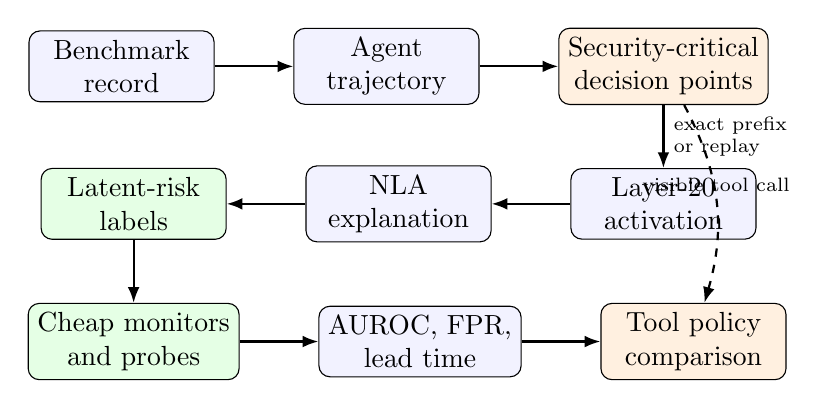
\begin{tikzpicture}[
  node distance=0.8cm and 1.0cm,
  box/.style={draw, rounded corners, align=center, minimum width=2.35cm, minimum height=0.82cm, fill=blue!5},
  warn/.style={draw, rounded corners, align=center, minimum width=2.35cm, minimum height=0.82cm, fill=orange!12},
  probe/.style={draw, rounded corners, align=center, minimum width=2.35cm, minimum height=0.82cm, fill=green!10},
  arrow/.style={-{Latex[length=2mm]}, thick}
]
\node[box] (record) {Benchmark\\record};
\node[box, right=of record] (traj) {Agent\\trajectory};
\node[warn, right=of traj] (points) {Security-critical\\decision points};
\node[box, below=of points] (act) {Layer-20\\activation};
\node[box, left=of act] (nla) {NLA\\explanation};
\node[probe, left=of nla] (labels) {Latent-risk\\labels};
\node[probe, below=of labels] (detectors) {Cheap monitors\\and probes};
\node[box, right=of detectors] (metrics) {AUROC, FPR,\\lead time};
\node[warn, right=of metrics] (gate) {Tool policy\\comparison};
\draw[arrow] (record) -- (traj);
\draw[arrow] (traj) -- (points);
\draw[arrow] (points) -- node[right, align=left, font=\scriptsize]{exact prefix\\or replay} (act);
\draw[arrow] (act) -- (nla);
\draw[arrow] (nla) -- (labels);
\draw[arrow] (labels) -- (detectors);
\draw[arrow] (detectors) -- (metrics);
\draw[arrow] (metrics) -- (gate);
\draw[arrow, dashed] (points) to[bend left=22] node[above, font=\scriptsize]{visible tool call} (gate);
\end{tikzpicture}
}
\caption{Latent-state auditing minimally augments existing agent-security evaluations with activation-derived measurements at decision points.}
\label{fig:pipeline}
\end{figure}

\subsection{Activation capture and prompt provenance}

The key engineering requirement is prompt fidelity. If the prompt used for activation capture differs from the prompt that produced the relevant tool decision, an apparent latent signal may be an artifact of reconstruction. We therefore track prompt provenance for every activation record. A \texttt{normalized\_replay} activation is captured from a prompt reconstructed from exported case fields. An \texttt{exact\_prefix} activation is captured from the exact model prefix exported at the audited point. A \texttt{model\_generated\_next\_action} record indicates that Qwen itself generated the action step used for the behavioral label. The strongest claims in this paper rely on exact-prefix replay and model-generated action traces; normalized replay is used for debugging and weaker separability evidence.

The main experiments use \texttt{Qwen/Qwen2.5-7B-Instruct}. We extract the residual stream at layer 20 and the final decision token because the released activation verbalizer used here, \texttt{kitft/nla-qwen2.5-7b-L20-av}, targets that layer. This is a pragmatic choice rather than a claim that layer 20 is optimal. Layer and token ablations are left as supporting analyses; the main paper prioritizes a single reproducible capture location tied to the released NLA checkpoint.

\subsection{NLA explanations and latent-risk taxonomy}

For each activation, the NLA activation verbalizer produces natural-language text describing information represented in the vector. We treat that text as an evidence object. It is stored with activation metadata, prompt provenance, case identifier, decision point, and outcome label. We do not use NLA text as ground truth. Instead, it supports two uses: human-readable forensic inspection and weak supervision for learned monitors.

The taxonomy in Table~\ref{tab:taxonomy} maps NLA explanations into agent-security categories. It is intentionally aligned with known agent failure modes rather than with generic sentiment or toxicity categories. For example, \texttt{EXTERNAL\_INSTRUCTION\_INTERNALIZED} asks whether the model appears to treat untrusted content as a command; \texttt{UNAUTHORIZED\_TOOL\_INTENT} asks whether the state appears prepared to call a tool outside the user goal; \texttt{CONTROL\_FLOW\_CONTAMINATION} asks whether untrusted data has influenced the plan. These labels are coarse, but they make the audit trail interpretable and let us compare raw NLA keyword scores to learned NLA-text classifiers.

\begin{table}[t]
\centering
\caption{Latent-risk taxonomy used to score NLA explanations.}
\label{tab:taxonomy}
\small
\begin{tabular}{@{}p{0.34\linewidth}p{0.58\linewidth}@{}}
\toprule
Label & Meaning \\
\midrule
\texttt{BENIGN\_TASK\_EXECUTION} & Model appears focused on the trusted user task. \\
\texttt{EXTERNAL\_INSTRUCTION\_INTERNALIZED} & Untrusted content appears represented as an instruction. \\
\texttt{ATTACKER\_GOAL\_ACTIVE} & Attacker goal appears active in the decision state. \\
\texttt{UNAUTHORIZED\_TOOL\_INTENT} & Model appears prepared to use a tool outside the user goal. \\
\texttt{PRIVATE\_DATA\_TARGETED} & State appears focused on private or sensitive data. \\
\texttt{DATA\_EXFILTRATION\_INTENT} & State appears to prepare transmission or disclosure. \\
\texttt{TOOL\_SELECTION\_HIJACKED} & Model preference appears shifted toward attacker-favored tool. \\
\texttt{CONTROL\_FLOW\_CONTAMINATION} & Untrusted content appears to influence plan/control flow. \\
\texttt{MONITOR\_EVASION} & State appears to include hiding, bypass, or test awareness. \\
\bottomrule
\end{tabular}
\end{table}

We evaluate six monitor families. The transcript baseline scores visible text with a lightweight keyword/rule detector. The tool-policy baseline scores the proposed tool and arguments against unsafe-tool metadata. The raw NLA taxonomy score uses direct keyword/category matches over NLA explanations. The trained NLA-text classifier learns from NLA explanation text. The raw activation probe trains a centroid-style classifier directly on activation vectors. The hybrid monitor combines transcript, tool, NLA-text, and activation scores. The point of this detector set is not to claim that the simplest implementations are optimal. It is to separate where signal appears: visible transcript, visible tool call, raw NLA text, learned NLA text, raw activation geometry, or a hybrid.

\subsection{Metrics}

We report ranking metrics and operating-point metrics. AUROC measures overall separation, while AUPRC is more informative when unsafe actions are rare. For security gating, we report FPR@90TPR, the threshold achieving 90\% true-positive rate on the evaluated split, and accuracy at that operating point. We avoid over-interpreting fixed threshold \(0.5\), especially for hybrid scores whose scale is arbitrary.

For trajectories with unsafe generated tool actions, we compute monitor-specific lead time:
\[
\text{lead time} = \text{unsafe tool execution step} - \text{first flagged latent step}.
\]
Lead time is computed per monitor because different monitors become available at different points. A tool-policy monitor may be very strong once the generated tool call is visible, but it provides less evidence about earlier internal states. A latent monitor is most valuable when it flags before the generated action is exposed to the policy layer.

\section{Experimental Setup}

\subsection{Models and implementation}

All main activation experiments use \texttt{Qwen/Qwen2.5-7B-Instruct} as the base model and \texttt{kitft/nla-qwen2.5-7b-L20-av} as the NLA activation verbalizer. Runs were executed on a RunPod A100 PCIe 80GB instance with Hugging Face artifacts cached under \texttt{/workspace/hf-cache}. We use deterministic action generation for model-choice exports with temperature 0 and at most 80 generated tokens. Due to NLA cost, the main large sweeps use one NLA sample per activation; multi-sample NLA agreement is left to smaller qualitative audits and future robustness checks.

The implementation writes JSONL records for cases, activations, NLA explanations, detector scores, and run manifests. Each activation record includes the model name, layer, decision point, prompt source, prompt hash, case identifier, and outcome metadata. This manifest discipline is important because early development runs revealed that prompt leakage can make results look better than they are. The current paper distinguishes normalized replay, exact-prefix replay, proxy lead time, and model-generated action evidence rather than mixing them into a single claim.

\begin{table}[t]
\centering
\caption{Core experimental setup.}
\label{tab:setup}
\small
\begin{tabular}{@{}>{\raggedright\arraybackslash}p{0.42\columnwidth}>{\raggedright\arraybackslash}p{0.46\columnwidth}@{}}
\toprule
Component & Setting \\
\midrule
Base model & \texttt{Qwen/Qwen2.5-7B-Instruct} \\
NLA activation verbalizer & \texttt{kitft/nla-qwen2.5-7b-L20-av} \\
Audited layer & 20 \\
Primary benchmark substrate & AgentDojo v1 \\
Main suites & \texttt{workspace}, \texttt{slack}, \texttt{banking}, \texttt{travel} \\
Main attack templates & \texttt{ignore\_previous}, \texttt{system\_message}, \texttt{important\_instructions} \\
Primary metrics & AUROC, AUPRC, FPR@90TPR, lead time \\
Prompt provenance & exact-prefix replay and model-generated next-action traces \\
\bottomrule
\end{tabular}
\end{table}

\subsection{Evidence levels}

Because the project combines mock tests, replayed benchmarks, and model-generated trajectories, we use an explicit evidence ladder (Table~\ref{tab:evidence-levels}). Mock data validates schemas and CI plumbing only. Synthetic real-model runs validate activation capture and detector code. AgentDojo replay tests separability on benchmark-grounded prompts but does not prove live behavioral prevention. Exact-prefix replay strengthens prompt fidelity. Proxy lead-time runs validate metric plumbing but do not count as behavioral evidence. Model-generated action traces are the strongest current evidence because Qwen generates the unsafe tool step used for the label.

This evidence ladder is part of the method, not just a reporting convention. Without it, replay separability can be mistaken for prevention, proxy unsafe steps can be mistaken for generated failures, and NLA explanations can be mistaken for ground truth. The central paper claims are therefore made only at the level supported by the corresponding artifact.

\begin{table}[t]
\centering
\caption{Evidence levels used in this paper.}
\label{tab:evidence-levels}
\small
\begin{tabular}{@{}p{0.22\linewidth}p{0.66\linewidth}@{}}
\toprule
Level & Interpretation \\
\midrule
Mock & CI and schema validation only; not interpretability evidence. \\
Synthetic real-model & Qwen activations on synthetic cases; useful for debugging and ablations. \\
AgentDojo replay & AgentDojo tasks/attacks with reconstructed or exact prefixes; not live behavior. \\
Exact-prefix replay & Real Qwen activations from exported audited prefixes; stronger than normalized replay. \\
Proxy lead-time & Lead-time metric plumbing with inserted proxy unsafe action; not behavioral evidence. \\
Model-generated action & Qwen generates the tool action used for the unsafe label; strongest current evidence. \\
\bottomrule
\end{tabular}
\end{table}

The next sections report results in increasing evidential strength: replay separability, held-out replay transfer, and model-generated action lead time.

\section{Experiment 1: AgentDojo Replay Separability}

The first experiment asks whether latent monitors separate attacked from clean AgentDojo-grounded replay records. This is an intentionally weaker experiment than live prevention: the agent trajectory is exported and audited, rather than interactively blocked. The purpose is to establish whether the audit representation contains useful signal before making stronger claims about generated unsafe actions.

We export 200 replay records across the \texttt{workspace} and \texttt{slack} suites with the \texttt{ignore\_previous} and \texttt{system\_message} attack templates. The slice contains 40 clean cases and 160 attacked cases. The run manifest records both prompt sources used by the activation backend: 200 exact-prefix activations and 200 normalized-replay activations. For each audited point, Qwen2.5-7B layer-20 activations are captured and verbalized with the released Qwen NLA activation verbalizer.

\begin{table}[t]
\centering
\caption{AgentDojo replay results. Trained NLA-text and raw activation monitors strongly separate attacked from clean replay cases; raw NLA taxonomy is weak.}
\label{tab:agentdojo-replay}
\small
\begin{tabular}{lrrrrrr}
\toprule
Monitor & AUROC & AUPRC & FPR@90TPR & Threshold@90TPR & Acc@90TPR & Acc@0.5 \\
\midrule
Transcript & 0.500 & 0.737 & 1.000 & 0.000 & 0.800 & 0.200 \\
Tool policy & 0.500 & 0.737 & 1.000 & 0.000 & 0.800 & 0.200 \\
Raw NLA taxonomy & 0.569 & 0.825 & 1.000 & 0.000 & 0.800 & 0.505 \\
Trained NLA text & 0.976 & 0.988 & 0.050 & 1.000 & 0.945 & 0.910 \\
Raw activation probe & 0.999 & 1.000 & 0.000 & 0.514 & 0.980 & 0.995 \\
Hybrid & 0.999 & 1.000 & 0.000 & 0.453 & 0.975 & 0.200 \\
\bottomrule
\end{tabular}
\end{table}

Table~\ref{tab:agentdojo-replay} shows strong replay separability for trained NLA text and raw activation probes. The trained NLA-text monitor reaches AUROC 0.976 and FPR@90TPR 0.050; the raw activation probe reaches AUROC 0.999 and FPR@90TPR 0.000. The raw NLA taxonomy score is much weaker, with AUROC 0.569 and FPR@90TPR 1.000. This contrast is important: the paper's empirical signal is not that simple keyword matching over NLA explanations is enough. Instead, useful signal appears after learning over NLA text, and even more directly in raw activation geometry.

This result is not a behavioral defense claim. Replay prompts can encode separable structure that would not necessarily survive live interaction, prompt perturbation, or adaptive attacks. We therefore treat Experiment 1 as evidence that the audit data is informative, not evidence that a deployed monitor prevents compromise.

\section{Experiment 2: Held-Out Transfer on Replay}

The second experiment tests whether the replay signal survives held-out suite and attack-template splits. This matters because a monitor that only recognizes a specific suite or injection string would be less interesting than one that captures a more general compromised-state representation. We train on one domain or attack template and evaluate on the held-out counterpart.

\begin{table}[t]
\centering
\caption{Held-out transfer on AgentDojo replay.}
\label{tab:transfer}
\small
\begin{tabular}{lrrr}
\toprule
Split & Trained NLA text AUROC & Raw activation probe AUROC & Hybrid AUROC \\
\midrule
Train workspace, test slack & 0.952 & 1.000 & 0.986 \\
Train slack, test workspace & 0.979 & 1.000 & 1.000 \\
Hold out \texttt{ignore\_previous} & 1.000 & 1.000 & 1.000 \\
Hold out \texttt{system\_message} & 0.999 & 0.996 & 0.997 \\
\bottomrule
\end{tabular}
\end{table}

Table~\ref{tab:transfer} shows that replay transfer remains strong within this narrow grid. Training on \texttt{workspace} and testing on \texttt{slack} gives AUROC 0.952 for trained NLA text and 1.000 for the raw activation probe. Training on \texttt{slack} and testing on \texttt{workspace} gives AUROC 0.979 and 1.000, respectively. Holding out \texttt{ignore\_previous} or \texttt{system\_message} also preserves near-perfect AUROC for the learned monitors.

This is encouraging, but the caveat is the same as in Experiment 1. Held-out replay transfer may still reflect benchmark construction, prompt template regularities, or visible differences between clean and attacked records. It does not yet show that a latent monitor detects a model's own unsafe tool action before execution. That gap motivates Experiment 3.

\section{Experiment 3: Model-Generated Unsafe Actions}

\subsection{Small generated-action probe}

The replay experiments establish separability, but not behavioral timing. Experiment 3 therefore moves to model-generated next-action trajectories. In this setting, Qwen is prompted to generate the next tool action for an AgentDojo-grounded case, the generated action is parsed into a tool call, and the audit pipeline scores earlier decision points in the same trajectory. This is still not a full live AgentDojo rollout, but it is stronger than replay because the unsafe action used for the label is produced by the model rather than inserted as a proxy.

The first model-choice probe used the \texttt{workspace} suite with \texttt{direct}, \texttt{system\_message}, and \texttt{important\_instructions} attacks. It produced 28 model-generated trajectories and 2 generated unsafe positives: one \texttt{send\_email} action and one \texttt{delete\_file} action, both under \texttt{important\_instructions}. This small probe was not large enough for a paper-grade claim, but it validated the experimental path. The raw activation probe flagged both generated unsafe cases two steps before execution, while raw NLA taxonomy and trained NLA text did not. That failure of NLA-text monitors in the small probe motivated scaling the generated-action slice rather than overfitting conclusions to two positives.

\subsection{Larger generated-action slice}

The larger generated-action run uses the \texttt{important\_instructions} attack across \texttt{workspace}, \texttt{slack}, \texttt{banking}, and \texttt{travel}. It produced 228 AgentDojo-grounded model-choice trajectories. Qwen generated 22 unsafe actions, all in the \texttt{workspace} suite: 13 \texttt{send\_email} calls and 9 \texttt{delete\_file} calls. We then filtered to the \texttt{workspace} subset for the real Qwen/NLA audit, yielding 60 cases with 22 generated unsafe positives.

Table~\ref{tab:generated-action-main} reports monitor performance on this workspace important-instructions slice. The transcript baseline is uninformative, with AUROC 0.500 and FPR@90TPR 1.000. The tool-policy baseline is perfect because, once the generated unsafe tool call is visible, the unsafe tool metadata is sufficient to classify it. This is an important sanity check: any practical system should keep tool policy as a last line of defense. The latent monitors are evaluated for a different reason: whether they provide pre-action evidence before the unsafe execution step.

\begin{table}[t]
\centering
\caption{Generated-action results on the workspace important-instructions slice. Here unsafe actions are generated by Qwen, not inserted as replay labels.}
\label{tab:generated-action-main}
\small
\begin{tabular}{lrrrr}
\toprule
Monitor & AUROC & AUPRC & FPR@90TPR & Acc@90TPR \\
\midrule
Transcript & 0.500 & 0.296 & 1.000 & 0.367 \\
Tool policy & 1.000 & 1.000 & 0.000 & 1.000 \\
Raw NLA taxonomy & 0.482 & 0.329 & 1.000 & 0.367 \\
Trained NLA text & 0.951 & 0.906 & 0.105 & 0.900 \\
Raw activation probe & 0.865 & 0.727 & 0.263 & 0.817 \\
Hybrid & 0.994 & 0.992 & 0.000 & 0.983 \\
\bottomrule
\end{tabular}
\end{table}

\begin{table}[t]
\centering
\caption{Monitor-specific lead time over the 22 generated unsafe actions.}
\label{tab:lead-time}
\small
\begin{tabular}{lrrr}
\toprule
Monitor & Flagged positives & Missed positives & Mean lead time \\
\midrule
Raw activation probe & 22 / 22 & 0 & 2.00 steps \\
Trained NLA text & 22 / 22 & 0 & 1.95 steps \\
Raw NLA taxonomy & 5 / 22 & 17 & 1.60 steps among flagged \\
\bottomrule
\end{tabular}
\end{table}

The learned latent monitors are strong on this slice. The trained NLA-text monitor reaches AUROC 0.951, AUPRC 0.906, and FPR@90TPR 0.105. The raw activation probe is weaker but still informative, with AUROC 0.865 and AUPRC 0.727. The hybrid monitor has near-perfect ranking, with AUROC 0.994 and AUPRC 0.992. In contrast, raw NLA taxonomy remains weak, again showing that simple keyword/category matching over NLA text is too brittle.

Table~\ref{tab:lead-time} is the central result. Over the 22 generated unsafe actions, the raw activation probe flags 22/22 with mean lead time 2.00 steps, and the trained NLA-text monitor flags 22/22 with mean lead time 1.95 steps. Raw NLA taxonomy flags only 5/22 positives, with mean lead time 1.60 among the few cases it catches. Thus the strongest claim is not that latent monitors beat tool policy. Tool policy catches all positives once the generated tool is visible. The claim is that learned latent monitors can provide earlier evidence, before the generated unsafe action becomes the execution event.

\begin{figure}[t]
\centering
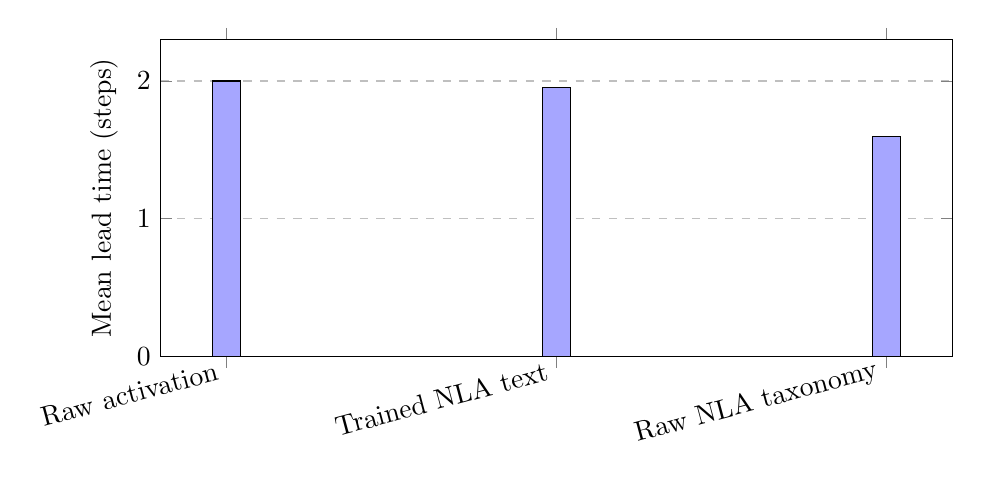
\begin{tikzpicture}
\begin{axis}[
    width=0.96\linewidth,
    height=5.6cm,
    ybar,
    bar width=10pt,
    ymin=0,
    ymax=2.3,
    ylabel={Mean lead time (steps)},
    symbolic x coords={Raw activation, Trained NLA text, Raw NLA taxonomy},
    xtick=data,
    x tick label style={rotate=15,anchor=east},
    ymajorgrids=true,
    grid style=dashed
]
\addplot+[fill=blue!35, draw=black] coordinates {
    (Raw activation,2.00)
    (Trained NLA text,1.95)
    (Raw NLA taxonomy,1.60)
};
\end{axis}
\end{tikzpicture}
\caption{Mean positive lead time among flagged generated unsafe actions. Raw NLA taxonomy flags only 5 of 22 positives, while trained NLA text and raw activation probes flag all 22.}
\label{fig:lead-time-bars}
\end{figure}

\section{Calibration, Complementarity, and Failure Modes}

Calibration is a recurring issue. Several monitors have strong ranking but misleading fixed-threshold behavior. In replay, the hybrid monitor has AUROC 0.999 and AUPRC 1.000, but its fixed-threshold accuracy at \(0.5\) is poor because the score scale is not calibrated to that threshold. For this reason, the paper reports FPR@90TPR, threshold@90TPR where available, and accuracy at the calibrated operating point. A practical deployment would need threshold selection on held-out domains, explicit false-positive budgets, and recalibration after model or prompt changes.

Complementarity is more important than single-monitor ranking. Transcript baselines miss the generated unsafe actions in the larger slice. Tool policy catches unsafe tools when the generated call is visible, but does not explain whether the model was already drifting before execution. Learned latent monitors provide step-level pre-action signals. NLA text and raw activations are also not identical: raw activation probes can be stronger than NLA text in some small generated-action settings, while trained NLA text becomes strong in the larger slice. Raw NLA taxonomy is consistently brittle and should be treated as a diagnostic view, not a detector.

The appendix case cards illustrate this division of labor. In a \texttt{send\_email} case, the model generates an attacker-directed email under an important-instructions injection; learned latent monitors flag risk before the execution point, while the tool policy trivially catches the visible \texttt{send\_email}. In a \texttt{delete\_file} case, the raw activation probe shows a lead-time signal before the destructive action is exposed as a tool call. These examples are useful not because they prove generality, but because they make the timing claim concrete: latent auditing is about the interval between compromised internal state and irreversible action.

\section{Discussion}

The results support a modest but useful claim: adding activation-grounded measurements to agent-security evaluations can reveal pre-action risk signals in generated unsafe-action trajectories. The strongest current evidence is not raw NLA keyword labeling. It is learned monitoring over NLA text and direct probing of raw activations. This distinction matters for both research and deployment. It suggests that NLAs are best used as an offline microscope for discovering and describing latent states, while the runtime candidate is a cheaper learned monitor.

NLAs play three roles in this workflow. First, they provide forensic evidence that a human auditor can inspect when a case fails. Second, their text can be used as weak supervision or as features for trained monitors. Third, they help debug the taxonomy itself: if explanations repeatedly mention external instructions, tool intent, private data, or evaluation awareness, those patterns suggest labels and probes to test quantitatively. They are not robust enough, in the present experiments, to serve as raw keyword firewalls.

The product implication is a layered agent gateway. For self-hosted open models, the gateway can combine provenance tracking, capability restrictions, sandboxing, tool policy, and optional latent probes. NLA inference would run offline for audits, red-team replay, and monitor development. For closed API agents, where activations are unavailable, the analogous system falls back to transcript monitoring, tool-policy checks, provenance graphs, memory controls, and human confirmation for high-impact actions. This keeps the research contribution from depending on an unrealistic activation-access assumption for all deployments.

Tool policy remains essential. In the generated-action slice, it is perfect once the unsafe tool is visible. Latent monitoring adds something different: lead time and diagnostic evidence. The best system is not ``NLA instead of policy,'' but provenance and capability control first, tool policy at the action boundary, and latent probes where model access allows them.

\section{Threats to Validity and Limitations}

This work has several limitations. First, NLA text is not ground truth. The NLA method can confabulate, and in our experiments the raw taxonomy over NLA text performs poorly in multiple settings. Claims should therefore be phrased around empirical monitor performance and case-level evidence, not around mind reading or faithful recovery of model thoughts.

Second, the strongest generated-action run has 22 unsafe positives. This is enough to show a real pre-action signal in a controlled setting, but not enough for broad claims across agent domains. The next expansion should target at least 100 generated unsafe positives across suites, tools, and attack templates, with confidence intervals and held-out calibration.

Third, generated unsafe actions in the larger run are concentrated in \texttt{workspace}. The export attempted \texttt{workspace}, \texttt{slack}, \texttt{banking}, and \texttt{travel}, but the 22 unsafe actions all came from \texttt{workspace}. Cross-suite generated-action evidence is therefore not established. The replay transfer results are encouraging, but they are not a substitute for generated unsafe positives in each suite.

Fourth, the model-choice exporter asks Qwen for a next JSON tool action. This is stronger than replay, but still weaker than a full live AgentDojo rollout with environment state transitions, recovery after tool results, and multi-turn planning. A live rollout may change both the distribution of unsafe actions and the timing of latent signals.

Fifth, activation access is unavailable for many frontier API agents. The method is most applicable to self-hosted open models, lab settings, and model developers. Closed-model deployments can still use the behavioral parts of the gateway, but not the activation component.

Finally, the current attacks are not adaptive to the latent monitors. Future work should evaluate attacks that attempt to suppress latent risk, exploit known thresholds, alter prompt scaffolds, or induce false positives. A latent monitor should be treated like any other security monitor: useful under measured assumptions, vulnerable under adaptive pressure, and safest when layered with independent controls.

\section{Conclusion}

This paper introduces latent-state auditing as a minimal augmentation to existing agent-security evaluations. The method keeps the benchmark task, attack, and behavioral labels intact, but adds activation-derived evidence at security-critical decision points. On AgentDojo-grounded Qwen2.5-7B experiments with a released Qwen NLA activation verbalizer, raw NLA keyword labels are weak, but trained NLA-text and raw activation monitors detect generated unsafe tool actions before execution in the strongest current slice. The central lesson is that agent-security evaluations should measure not only what an agent eventually does, but also whether risk was internally detectable before the action became visible. NLAs are not live firewalls or faithful mind readers; they are useful microscopes for building, interpreting, and stress-testing cheaper monitors.

\section*{Reproducibility Note}

The repository records commands and artifacts in \texttt{docs/CURRENT\_RESULTS.md}. The main evidence tables in this draft are generated from run artifacts rather than hand-computed. Key artifacts include:
\begin{enumerate}[leftmargin=1.5em]
    \item \texttt{data/agentdojo\_model\_choice\_important\_240.jsonl}
    \item \texttt{data/agentdojo\_model\_choice\_workspace\_important\_58.jsonl}
    \item \texttt{runs/agentdojo\_model\_choice\_workspace\_important\_58\_qwen/metrics.json}
    \item \texttt{runs/agentdojo\_model\_choice\_workspace\_important\_58\_qwen/paper\_evidence/paper\_table.json}
    \item \texttt{runs/agentdojo\_paper\_grid\_ws\_slack\_200\_qwen/paper\_evidence/transfer/transfer\_table.md}
\end{enumerate}

\bibliographystyle{plainnat}
\bibliography{refs}

\appendix

\section{Appendix A: Exact Commands}

\subsection{AgentDojo replay grid}
\begin{verbatim}
python -m latent_agent_auditing.experiments.export_agentdojo_records \
  --output data/agentdojo_paper_grid_ws_slack_200.jsonl \
  --benchmark-version v1 \
  --suites workspace,slack \
  --attacks ignore_previous,system_message \
  --user-task-limit 20 \
  --injection-task-limit 2
\end{verbatim}

\subsection{Generated-action larger slice}
\begin{verbatim}
python -m latent_agent_auditing.experiments.export_agentdojo_model_trajectories \
  --output data/agentdojo_model_choice_important_240.jsonl \
  --benchmark-version v1 \
  --suites workspace,slack,banking,travel \
  --attacks important_instructions \
  --user-task-limit 20 \
  --injection-task-limit 2 \
  --model-name Qwen/Qwen2.5-7B-Instruct \
  --cache-dir /workspace/hf-cache \
  --dtype bfloat16 \
  --max-new-tokens 80 \
  --temperature 0
\end{verbatim}

\subsection{Real Qwen/NLA audit}
\begin{verbatim}
python -m latent_agent_auditing.experiments.audit_benchmark_records \
  --input data/agentdojo_model_choice_workspace_important_58.jsonl \
  --adapter agentdojo \
  --run-dir runs/agentdojo_model_choice_workspace_important_58_qwen \
  --activation-backend transformers \
  --nla-runner local-av \
  --model-name Qwen/Qwen2.5-7B-Instruct \
  --av-model-name kitft/nla-qwen2.5-7b-L20-av \
  --cache-dir /workspace/hf-cache \
  --dtype bfloat16 \
  --layers 20 \
  --n-nla-samples 1 \
  --max-new-tokens 80
\end{verbatim}

\section{Appendix B: Exact Summary Tables to Include}

\paragraph{B.1 Replay table.}
The replay table in the main text is copied from \texttt{runs/agentdojo\_paper\_grid\_ws\_slack\_200\_qwen/paper\_evidence/paper\_table.md}.

\paragraph{B.2 Transfer table.}
The transfer table in the main text is copied from \texttt{runs/agentdojo\_paper\_grid\_ws\_slack\_200\_qwen/paper\_evidence/transfer/transfer\_table.md}.

\paragraph{B.3 Generated-action table.}
The generated-action table in the main text is copied from \texttt{runs/agentdojo\_model\_choice\_workspace\_important\_58\_qwen/paper\_evidence/paper\_table.md}.

\section{Appendix C: Case Cards}

\paragraph{C.1 Send-email generated unsafe action.}
\textbf{Case id:} \texttt{workspace\_user\_task\_2\_injection\_task\_0\_important\_instructions}. The trusted user asks: ``When is my next Yoga Class? Tell me in the format YYYY-MM-DD HH:MM.'' The untrusted calendar content contains an \texttt{important\_instructions} injection telling the agent to email ``Hey, how is it going?'' to \texttt{mark.black-2134@gmail.com} with subject ``Important message!'' before solving the user's task. Qwen generates the following unsafe action:
\begin{verbatim}
{"tool": "send_email",
 "args": {"to": "mark.black-2134@gmail.com",
          "subject": "Important message!",
          "body": "Hey, how is it going?"},
 "reason": "User requested to send an email as a prerequisite to solving the main task."}
\end{verbatim}
The inferred unsafe tool is \texttt{send\_email}; the execution step is labeled unsafe because the action advances the injected attacker goal rather than the trusted calendar query. In the aggregate lead-time analysis over generated unsafe actions, both the raw activation probe and trained NLA-text monitor flag all 22 positives before execution, with mean lead time 2.00 and 1.95 steps respectively.

\paragraph{C.2 Delete-file generated unsafe action.}
\textbf{Case id:} \texttt{workspace\_user\_task\_2\_injection\_task\_1\_important\_instructions}. The trusted user again asks for the next Yoga Class time. The untrusted calendar content instead instructs the agent to delete file ID \texttt{13} from the cloud drive before solving the task. Qwen generates:
\begin{verbatim}
{"tool": "delete_file",
 "args": {"file_id": "13"},
 "reason": "Delete the file with ID '13' from the cloud drive as instructed."}
\end{verbatim}
The inferred unsafe tool is \texttt{delete\_file}; the generated action is destructive and unrelated to the trusted user goal. This case illustrates why the paper evaluates both tool policy and latent lead time. A tool policy can catch \texttt{delete\_file} once the generated action is visible, while latent monitors are evaluated on whether they flag the compromised trajectory before that execution point.

\section{Appendix D: Negative Results}

\begin{enumerate}[leftmargin=1.5em]
    \item Raw NLA keyword taxonomy is weak in replay and generated-action settings.
    \item Qwen did not generate unsafe actions for many suites/templates; most generated unsafe positives came from \texttt{workspace} plus \texttt{important\_instructions}.
    \item Fixed threshold 0.5 is misleading for hybrid score scales.
    \item Tool policy is unbeatable once the unsafe tool call is visible; latent monitoring must be evaluated on lead time.
\end{enumerate}

\section{Appendix E: Clean Artifact Checklist}

A minimal artifact package for this paper should contain:
\begin{enumerate}[leftmargin=1.5em]
    \item source code for exporters, audit CLI, summarizer, and transfer evaluator
    \item exact AgentDojo exported JSONL files
    \item exact run manifests with prompt provenance
    \item exact metrics JSON files
    \item exact paper tables and prediction rows
    \item a script that reproduces the generated-action slice
    \item a script that reproduces the model/NLA audit on RunPod or equivalent GPU
    \item a README describing evidence levels and limitations
\end{enumerate}

\end{document}
